\subsection{Porte TTL e scheda di visualizzazione}
Le porte logiche a tecnologia TTL funzionano utilizzando come 1 logico il valore di tensione +\SI{5}{\volt} mentre come 0 logico \SI{0}{\volt}. Per controllare il funzionamento dei nostri circuiti utilizzeremo una schedina di visualizzazione a led. Tale circuito permette di visualizzare lo stato "alto" o "basso" delle linee da monitorare tramite 8 led (4 rossi e 4 verdi). Tali schede contengono un integrato buffer 74LS244 nella logica TTL che fornisce in uscita una corrente di \SI{-15}{\milli\ampere} per il livello alto e di \SI{24}{\milli\ampere} per il livello basso.
Ricordiamo che l'alimentazione deve essere stabilizzata e disaccoppiata con i condensatori come nel caso analogico in quanto nei momenti di commutazione delle porte abbiamo grandi variazioni di tensione in piccoli tempi (idealmente la variazione da stato 1 a 0 è istantanea). È dunque essenziale avere una riserva di cariche utilizzabili dal circuito nel momento in cui si hanno commutazioni.

\subsubsection{Porta NAND}

\begin{wrapfigure}[5]{r}{0.45\textwidth}
\centering
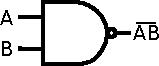
\includegraphics[width=.15\textwidth]{../E09/latex/NAND.pdf}
\caption{Simbolo circuitale convenzionalmente utilizzato per porte NAND.}
\label{cir9:nand}
\end{wrapfigure}

Abbiamo verificato il funzionamento di una porta NAND utilizzando, come già detto, una scheda di visualizzazione a LED. È stata verificata la seguente tavola di verità. 



\begin{tabular}{|l|l|l|}
\hline
A & B & $\overline{AB}$ \\
\hline
0 & 0 & 1\\
\hline
0 & 1 & 1\\
\hline
1 & 0 & 1\\
\hline
1 & 1 & 0\\
\hline
\end{tabular}

\subsubsection{Porta NOT}


\begin{wrapfigure}[10]{r}{0.35\textwidth}
\centering
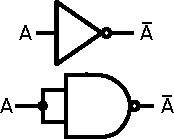
\includegraphics[width=.15\textwidth]{../E09/latex/NOT.pdf}
\caption{Implementazione e simbolo circuitale per porte NOT.}
\label{cir9:not}
\end{wrapfigure}


Non avendo a disposizione una porta NOT, abbiamo utilizzato una porta NAND cortocircuitando i due ingressi tra loro. Così facendo otteniamo un'implementazione di una porta NOT. Ne abbiamo in primis verificato il funzionamento collengandola alla scheda di visualizzazione led e fornendo un'onda quadra in ingresso ($V_{pp}=\SI{5}{\volt}$, $V_{off}=+\SI{2.5}{\volt}$, $\nu=\SI{2}{\hertz}$). Una volta verificato funzionasse, collegato ingresso ed uscita all'oscilloscopio e ne abbiamo analizzato la risposta per diverse tensioni costanti in ingresso. I dati ottenuti sono riportati in Tabella (\ref{tab9:risposta}). Come vediamo, tra \SI{1}{\volt} e \SI{1.5}{\volt} la tensione varia in modo molto rapido.

Siamo dunque interessati a capire meglio la risposta della porta in funzione della tensione in ingresso. Per fare ciò ci aiuta l'oscilloscopio con la modalità XY.  




\begin{tabular}{|l|l|||l|l|||l|l|||l|l|}
\hline
$V_{in}$ [\si{\volt}] & $V_{out}$ [\si{\volt}] & $V_{in}$ [\si{\volt}]& $V_{out}$ [\si{\volt}] & $V_{in}$ [\si{\volt}]& $V_{out}$ [\si{\volt}] & $V_{in}$ [\si{\volt}]& $V_{out}$ [\si{\volt}]\\
\hline
0 & 4.30 & 2.5 & 0.10 & 5  & 0.10 & 2.5 & 0.10\\
\hline
0.5 & 4.05 & 3 & 0.10 & 4.5 & 0.10 & 2 &0.10\\
\hline
1 & 3.01 & 3.5 & 0.10 & 4 & 0.10 & 1.5 & 0.10\\
\hline
1.5 & 0.10 & 4 & 0.10 & 3.5 & 0.10 & 1 & 3.00\\
\hline
2 & 0.10 & 4.5 & 0.10 & 3.0 &0.10 & 0.5 & 4.05\\
\hline
\label{tab9:risposta}
\end{tabular}


Abbiamo dunque fornito un'onda sinusoidale all'ingresso di frequenza \SI{100}{\kilo\hertz}, $V_{pp}=\SI{5}{\volt}$ e $V_{off}=+\SI{2.5}{\volt}$. Come vediamo dal grafico sotto riportato, sebbene stiamo lavorando con segnali digitali (1 o 0) le tensioni in gioco sono manifestamente analogiche. Avremo dunque tutta la serie di problemi già affrontati nella parte analogica del corso. Vediamo infatti che la tensione in uscita non è una funzione a gradino. Inoltre, per evitare che rumori molesti disturbino il segnale in uscita, avremo bisogno di una sorta di isteresi. Non esisterà dunque un valore ben definito di V alta e V bassa, ma delle bande di lavoro. Solitamente nel data-shit sono riportati tali parametri.

$$GRAFICO$$

\subsubsection{Circuito di GATE con porta AND}
Per realizzare il circuito GATE è sufficiente utilizzare una porta AND con un segnale di controllo ad un ingresso. Per realizzare una porta AND possiamo utilizzare 2 NAND come proposto nella seguente figura. Infatti, utilizzando la notazione convenzionale, $AB=\overline {\overline {AB}}$ che trivialmente è una NAND e una NOT in serie.
 
\begin{wrapfigure}[10]{r}{0.35\textwidth}
\centering
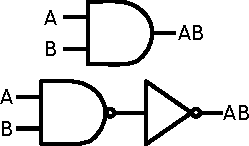
\includegraphics[width=.15\textwidth]{../E09/latex/AND.pdf}
\caption{Implementazione e simbolo circuitale per porte AND.}
\label{cir9:and}
\end{wrapfigure}

La tavola di verità è la seguente (C=controllo, S=segnale):

\begin{tabular}{|l|l|l|}
\hline
C & S & CS \\
\hline
0 & 0 & 0\\
\hline
0 & 1 & 0\\
\hline
1 & 0 & 0\\
\hline
1 & 1 & 1\\
\hline
\end{tabular}

Come vediamo dalla tabella, se il segnale di controllo è a 0 logico l'uscita sarà sempre 0 logico. Se invece il controllo è a 1 logico, allora l'uscita sarà una copia del segnale in ingresso. Per verificare ciò, abbiamo collegato l'oscilloscopio all'uscita del circuito e fornito un'onda quadra ($V_{pp}=\SI{5}{\volt}$, $V_{off}=+\SI{2.5}{\volt}$, $\nu=\SI{2}{\hertz}$). Abbiamo visto che quando il controllolol era collegato a comune, l'uscita era praticamente nulla. Nell'altro caso invece avevamo la stessa onda quadra dell'ingresso anche all'uscita.

\subsubsection{Porta XOR}

Una porta XOR implementa la funzione matematica della somma diretta. Avendo solo a disposizione porte NAND, dobbiamo cercare di implementare un circuito che svolga tale funzione. Riportiamo in tabella la tavola di verità. In questo semplice caso non è necessario scomodare dalla tomba il povero Karnaugh.

\begin{tabular}{|l|l|l|}
\hline
A & B & $A \oplus B$ \\
\hline
0 & 0 & 0\\
\hline
0 & 1 & 1\\
\hline
1 & 0 & 1\\
\hline
1 & 1 & 0\\
\hline
\end{tabular}

\begin{wrapfigure}[15]{r}{0.35\textwidth}
\centering
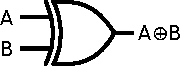
\includegraphics[width=.30\textwidth]{../E09/latex/XOR.pdf}
\caption{Implementazione e simbolo circuitale per porte XOR.}
\label{cir9:xor}
\end{wrapfigure}

Dunque $A \oplus B=A\overline B + \overline A B$, dove con A,B indichiamo l'1 logico, con $\overline A,\overline B$ lo 0 logico.

Applichiamo le regole di somme e prodotti viste a lezione:

$$A \oplus B=A\overline B + \overline A B=\overline{\overline{A\overline B + \overline A B}}=\overline{\overline{A\overline B} \cdot \overline{\overline A B}}$$

Dunque, il circuito per realizzare uno XOR usando porte NAND e NOT è il seguente.



Come vediamo, la realizzazione da noi progettata prevede l'utilizza do 2 porte NOT e 3 NAND. Ne abbiamo verificato il funzionamento con la solita scheda a LED.





\subsubsection{Votazione con 3 Giurati e 1 Presidente}
Il circuito di votazione di 3 Giurati con 1 Presidente prevede di sommare i voti dei vari membri tenendo però in considerazione che il voto del presidente vale doppio. Partiamo dunque dalla mappa di Karnaugh.


\begin{tabular}{|l|l|l|l|l|}
\hline
\diaghead{\theadfont lololololo a} {CP}{AB}& 00& 01 & 11&10\\
\hline
00&0 & 0 & 0 &0 \\
\hline
01&0 & 1 & 1 &1 \\
\hline
11&1 &1  &1  &1 \\
\hline
10&0 & 0 & 1 & 0\\

\hline

\end{tabular}




Ora, minimizzando tale mappa otteniamo $Y=ABC+P(A+B+C)$. Come fatto prima, avendo a disposizione solo porte NAND, trasformiamo tutto in prodotti.

$$Y=ABC+P(A+B+C)=\overline{\overline{ABC+P(A+B+C)}}=\overline{\overline{ABC} \cdot \overline {P(A+B+C)} }= \overline{\overline{(AB)C} \cdot \overline {P(\overline{\overline{{A+B+C}} })}}=\overline{\overline{(AB)C} \cdot \overline {P(\overline{{(\overline A \cdot \overline B) \cdot \overline C} })}}$$

Ora è immediato costruire il circuito utilizzando porte NAND e NOT. Lo schema è riportato in figura. Come per gli altri circuiti, è stato verificato utilizzando la schedina a LED. 



\begin{figure}[htpc]
\centering
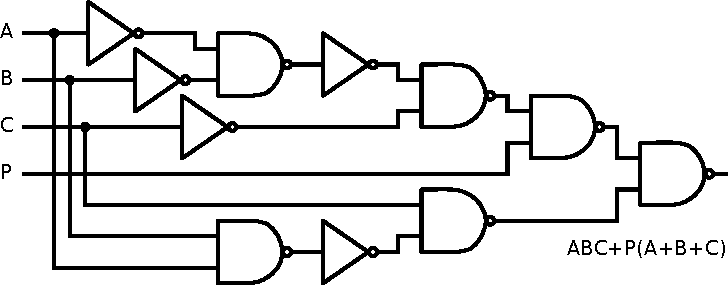
\includegraphics[width=.75\textwidth]{../E09/latex/giudici.pdf}
\caption{Buzz non ha capito che sono 3 giurati e 1 giudice, non 4 giudici.}
\label{cir9:giudici}
\end{figure}


\subsubsection{Allarme MINI-APPARTAMENTO}

In quest'ultima parte dell'esperienza cercheremo di progettare e costruire un circuito di allarme. Immaginiamo di avere una villa piena di zoccole e di aver installato dei sensori. Vogliamo analizzarne i segnali per decidere se l'allarme deve suonare o no. Chiamiamo P il sensore sulla porta (0=chiusa), F il sensore sulla finestra (0=chiusa), I il sensore ad infrarossi (0=no movimento) e infine C la chiave che permette di attivare l'allarme escludendo il sensore ad infrarossi (1=escludo infrarossi). 

Costruiamoci la mappa di Karnaugh.


\begin{tabular}{|l|l|l|l|l|}
\hline
\diaghead{\theadfont lololololo a} {IC}{PF}& 00& 01 & 11&10\\
\hline
00&0 & 1 & 1 &1 \\
\hline
01&0 & 1 & 1 &1 \\
\hline
11&0 &1  &1  &1 \\
\hline
10&1 & 1 & 1 & 1\\

\hline

\end{tabular}

Trivialmente, una dei possibili raggruppamenti è il seguente $Y=P+F+\overline C I$. Con la ormai nota tecnica trasformiamo tutto in NAND e NOT.

$$Y=P+F+\overline C I=\overline{\overline{P+F+\overline C I}}=\overline{(\overline P \cdot \overline F) \cdot \overline{\overline C I}}$$ 

Il circuito risulta quello nella seguente figura. È stato verificato come gli altri utilizzando la scheda a LED.



\begin{figure}[htpc]
\centering
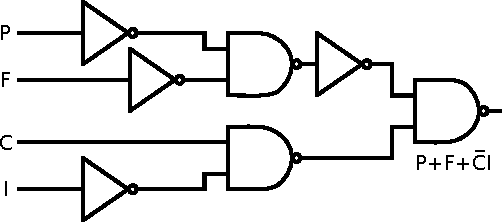
\includegraphics[width=.65\textwidth]{../E09/latex/allarme.pdf}
\caption{Bisogna negare il C, non I.}
\label{cir9:allarme}
\end{figure}







